      
               
                \begin{ledgroupsized}[r]{120mm}
                \footnotesize 
                \pstart                
                \noindent\textbf{\"{U}berlieferung:}   
                \pend
                \end{ledgroupsized}
            
              
                            \begin{ledgroupsized}[r]{114mm}
                            \footnotesize 
                            \pstart \parindent -6mm
                            \makebox[6mm][l]{\textit{L}}Konzept: LH XXXVII 3 Bl. 91\textendash96. 3 Bog. 2\textsuperscript{o}. 10 1/4 S. zweispaltig. Bl. 96~r\textsuperscript{o} sowie 1/4 von Bl. 96~v\textsuperscript{o} N.~63. Bl. 91 r\textsuperscript{o}\textendash95 r\textsuperscript{o} linke Spalte beschrieben. In der rechten Spalte Erg\"{a}nzungen und Textkorrekturen. Auf Bl. 91 v\textsuperscript{o} in der rechten Spalte eine Zeichnung, deren Zuordnung zum Text unklar ist. Auf Bl. 95 v\textsuperscript{o} beginnt in der rechten Spalte oben eine Marginalie, die in der linken Spalte unter dem Haupttext fortgesetzt wird und auf Bl. 96 v\textsuperscript{o} endet. Aufgrund ihrer Länge und der Tatsache, dass sie unmittelbar an den letzten Satz des Haupttextes anschließt, wird sie als Fortsetzung des Textes behandelt.\\Cc 2, Nr. 486 A tlw. \pend
                            \end{ledgroupsized}
                %\normalsize
                \vspace*{5mm}
                \begin{ledgroup}
                \footnotesize 
                \pstart
            \noindent\footnotesize{\textbf{Datierungsgr\"{u}nde}: Leibniz bezieht sich in dem vorliegenden Text des \"{O}fteren auf den Huygens-Brief, der im \cite{00062}\textit{Journal des S\c{c}avans} vom 25. Juli 1672 ver\"{o}ffentlicht wurde. Da diese Ausgabe der Zeitschrift in dem vorliegenden St\"{u}ck als die zuletzt erschienene bezeichnet wird, muss der Text in der Zeit zwischen dem 25. Juli und dem 12. Dezember 1672 (dem Erscheinungsdatum der n\"{a}chsten Nummer) verfasst worden sein. Wir \"{u}bernehmen diesen Zeitraum daher als Entstehungszeit des vorliegenden St\"{u}ckes.}
                \pend
                \end{ledgroup}
            
                \vspace*{8mm}
                \pstart 
                \normalsize
            [91 r\textsuperscript{o}] \selectlanguage{latin}Experimenta\protect\index{Sachverzeichnis}{experimentum!pneumaticum} \edtext{novissima Pneumatica}{\lemma{}\Afootnote{novissima Pneumatica \textit{ erg.} \textit{ L}}} Illustris Hugenii\protect\index{Namensregister}{\textso{Huygens} (Hugenius, Vgenius, Hugens, Huguens), Christiaan 1629\textendash 1695}, novam quandam velut  portam nobis aperuere in interiora naturae. Hactenus enim  ratiocinatione tantum assecuti sumus, nunc etiam experientia deprehendimus,  corpus quoddam ipso aere communi subtilius, Recipienti\protect\index{Sachverzeichnis}{Recipiens!Magdeburgicum} \edtext{Magdeburgico sive}{\lemma{}\Afootnote{Magdeburgico sive \textit{ erg.} \textit{ L}}} Antliae Pneumaticae\protect\index{Sachverzeichnis}{antlia!pneumatica} inesse, sive id ex ipso aere communi \edtext{per suctionem}{\lemma{per suctionem}\Afootnote{\textit{ erg.} \textit{ L}}}  attenuato productum \edtext{aut segregatum}{\lemma{}\Afootnote{aut segregatum \textit{ erg.} \textit{ L}}}, sive per poros vitri illapsum sit. \edtext{Sed ut haec}{\lemma{sit.}\Afootnote{ \textit{ (1) }\ Quamquam id corpus  \textit{(a)}\ adhuc longe absit a \textit{(b)}\ longe lateque differre  necesse sit a materia subtili\protect\index{Sachverzeichnis}{materia!subtilis|textit} primi secundive gradus, Cartesiana\protect\index{Sachverzeichnis}{materia!Cartesiana|textit}   \textbar\ sunt tamen circa horum Experimentorum \textit{ erg.}\ \textbar\ , quae ut \textit{ (2) }\ Sed ut haec \textit{ L}}} agnoscantur distinctius primum consequentias quasdam ex his Phaenomenis ducam, deinde rationes eorum afferre conabor. Et primum \edtext{sequitur}{\lemma{primum}\Afootnote{ \textit{ (1) }\ demonstratur \textit{ (2) }\ sequitur \textit{ L}}}, hinc \edtext{\textso{Recipientem}\protect\index{Sachverzeichnis}{Recipiens!Magdeburgicum}\textso{ Magdeburgicum (aut etiam summitatem Tubi Torricelliani)}}{\lemma{\textso{Recipientem}}\Afootnote{ \textit{ (1) }\ \textso{Antliae Pneumaticae}\protect\index{Sachverzeichnis}{antlia!pneumatica|textit} \textit{ (2) }\ \textso{Magdeburgicum [...] Torricelliani)} \textit{ L}}}\textso{ non esse }\edtext{\textso{omni corpore }}{\lemma{\textso{esse}}\Afootnote{ \textit{ (1) }\ \textso{vacuum} \textit{ (2) }\ \textso{omni corpore vacua} \textit{ L}}}\textso{vacua.}\footnote{An in summitate Tubi Torricelliani\protect\index{Sachverzeichnis}{Tubus!Torricellianus} vacua experimentum instituendum.}%
\edtext{ Nam quod duae laminae politae sibi invicem  accommodatae sine ullo vinculo sensibili}{\lemma{\textso{vacua.}}\Afootnote{ \textit{ (1) }\ Necesse est enim  utique pressioni cuidam ascribi, quod duae laminae politae\protect\index{Sachverzeichnis}{laminae politae|textit} sine sustentaculo vinculoque sensibili \textit{ (2) }\ Nam [...] sensibili \textit{ L}}}  resistunt divellenti, id necesse est  aut a vinculo quodam insensibili seu causa unionis inter  ipsas laminas\protect\index{Sachverzeichnis}{laminae politae}; aut ab externa quadam causa laminas\protect\index{Sachverzeichnis}{laminae politae} \edtext{continente}{\lemma{laminas}\Afootnote{ \textit{ (1) }\ comprimente \textit{ (2) }\ continente \textit{ L}}} oriri. Sed a vinculo inter ipsas laminas\protect\index{Sachverzeichnis}{laminae politae}  oriri non potest, id enim non tantum divulsioni, sed et motioni  parallelae resisteret, qua laminae\protect\index{Sachverzeichnis}{laminae politae} facile separantur. Necesse  est ergo corpus \edtext{duas laminas continens aut potius ne divellantur impediens}{\lemma{corpus}\Afootnote{ \textit{ (1) }\ comprimens \textit{ (2) }\ duas laminas  \textit{(a)}\ comprimens \textit{(b)}\ continens [...] impediens \textit{ L}}} statui, etiam in Recipiente Magdeburgico\protect\index{Sachverzeichnis}{Recipiens!Magdeburgicum},  utcunque exhausto. Quare \edtext{ ipsum Celeberrimum Gerickium nostrum  cui Respublica literaria illustris illius Experimenti Pneumatici primam inventionem debet  vacuo, quod vocat, summo omni corpore spoliato}{\lemma{Quare}\Afootnote{ \textit{ (1) }\ nescio an Celeberrimus Gerickius\protect\index{Namensregister}{\textso{Guericke} (Gerickius, Gerick.), Otto v. 1602\textendash 1686|textit} noster  cui Respublica literaria primum in haec experimenta aditum  debet vacuum, quod vocat, summum omni corpore spoliatum sustinere \textit{ (2) }\ ipsum [...] Pneumatici  \textbar\ ad \textit{ gestr.}\ \textbar\ primam [...] spoliato \textit{ L}}}  visis his experimentis, quo est candore, renuntiaturum credo.\pend  
                        \pstart 
                         Sequitur \textso{secundo corpus in }\textso{Recipiente Magdeburgico}\protect\index{Sachverzeichnis}{Recipiens!Magdeburgicum}\textso{ residuum  nihilominus esse crassum.} \textso{Crassum} voco quod a corporibus\protect\index{Sachverzeichnis}{corpus!sensibile}  sensibilibus aut omnino retinetur, aut non nisi cum difficultate \edtext{transmittitur. Haec propositio}{\lemma{transmittitur.}\Afootnote{ \textit{ (1) }\ Nam si corpus illud \textit{ (2) }\ Haec propositio \textit{ L}}} \edtext{ex altero}{\lemma{propositio}\Afootnote{ \textit{ (1) }\ non quidem  ex \textit{ (2) }\ ex altero \textit{ L}}} \edtext{aquae aut Mercurii}{\lemma{altero}\Afootnote{ \textit{ (1) }\ Aquae in Tubo Torri \textit{ (2) }\ aquae aut Mercurii \textit{ L}}}  ab aere purgati et solito altius suspensi experimento conficitur. Nam si \edtext{corpus illud invisibile in fig. Diarii p. 134\edtext{}{\lemma{134}\Bfootnote{\textsc{Chr. Huygens, }\cite{00062}\textit{Extrait d'une lettre}, \textit{JS} (1672), S.~134 (\textit{HO} VII, S.~202).\protect\rule[0cm]{1.5cm}{0cm}}} quod vas \textit{B} aere exhaustum implet summa facilitate per  medium Mercurii aquaeve corpus aut in vase \textit{D} aut tubi \textit{C} per commissuram inter  aquam aut Mercurium lateraque vasis \textit{D} et tubi \textit{C} pervaderet;}{\lemma{si}\Afootnote{ \textit{ (1) }\ summa facilitate pervaderet corpus illud \textit{ (2) }\ corpus [...] 134 \textit{(a)}\ vas \textit{B} implens \textit{(b)}\ quod [...] aut \textit{(aa)}\ per commissuram inter  aquam aut Mercurium\protect\index{Sachverzeichnis}{mercurius|textit} lateraque Tubi, \textit{(bb)}\ in vase \textit{D} aut  \textit{(aaa)}\ phiala \textit{C} \textit{(bbb)}\ tubi [...] et \textit{(aaaa)}\ phiala \textit{(bbbb)}\ tubi \textit{C} pervaderet; \textit{ L}}} utique nulla \edtext{esset ratio quae aquam aut Mercurium  suspenderet}{\lemma{esset}\Afootnote{ \textit{ (1) }\ aquae aut Mercurii\protect\index{Sachverzeichnis}{mercurius|textit} suspen \textit{ (2) }\ ratio [...] suspenderet \textit{ L}}} \edtext{in Tubo \textit{C} ultra perpendiculum vasis \textit{D}}{\lemma{in}\Afootnote{Tubo \textit{C} ultra perpendiculum vasis \textit{D} \textit{ erg.} \textit{ L}}}, nam spatium\edtext{}{\lemma{}\Afootnote{spatium  \textbar\ ab \textit{ gestr.}\ \textbar\ eorum \textit{ L}}} eorum descensu in Tubo relictum  facile a corpore isto \edtext{omnia penetrante impleretur}{\lemma{isto}\Afootnote{ \textit{ (1) }\ vel impellatur, cum aqua aut \textit{ (2) }\ omnia penetrante impleretur \textit{ L}}}. Quemadmodum\edtext{}{\lemma{}\Afootnote{Quemadmodum  \textbar\ enim \textit{ gestr.}\ \textbar\ lamina \textit{ L}}} lamina lata ex materia \edtext{licet}{\lemma{}\Afootnote{licet \textit{ erg.} \textit{ L}}} aqua graviore \edtext{parata}{\lemma{}\Afootnote{parata \textit{ erg.} \textit{ L}}} nihilominus  in aqua \edtext{natat}{\lemma{aqua}\Afootnote{ \textit{ (1) }\ natare potest \textit{ (2) }\ natat \textit{ L}}}, at si cribri instar perforetur, \edtext{quia}{\lemma{perforetur,}\Afootnote{ \textit{ (1) }\ cum scilicet \textit{ (2) }\ quia \textit{ L}}} aqua per foramina in summum evadere potest,  mergitur. Quare corpus hoc subtile cujuscunque tandem sit naturae,  certe a Cartesianorum Elementorum\protect\index{Sachverzeichnis}{elementum Cartesianum} primi secundique \edtext{subtilitate}{\lemma{}\Afootnote{subtilitate \textit{ erg.} \textit{ L}}} longe abest;  quibus ille luminis\protect\index{Sachverzeichnis}{lumen} magnetisque\protect\index{Sachverzeichnis}{magnes} actionem \edtext{ corpora durissima facile penetrantem, explicat.}{\lemma{actionem}\Afootnote{ \textit{ (1) }\ explicat, quae  constat etiam corpora durissima summa facilitate  \textit{(a)}\ transire \textit{(b)}\ penetrare. \textit{ (2) }\  corpora durissima facile penetrantem, explicat. \textit{ L}}}\pend 
%                         \begin{center}                   
%                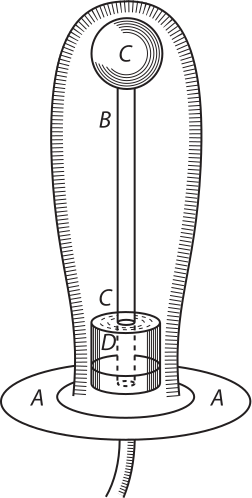
\includegraphics[width=0.3\textwidth]{images/37_3_91r}\\\textit{[Fig. 1, nach Chr. Huygens, \cite{00062}Extrait d'une lettre ergänzt]}
%                        %\caption{Bildbeschreibung}
%                       \end{center} 
                         \pstart  Sequitur 3\textsuperscript{tio} \textso{suspensionem }\textso{Mercurii}\protect\index{Sachverzeichnis}{mercurius}\textso{ aquaeve ultra }\edtext{\textso{solitum non magis corpori illi aere subtiliori, quam ipsi  aeri adscribendam.}}{\lemma{\textso{solitum}}\Afootnote{ \textit{ (1) }\ \textso{non oriri} \textit{ (2) }\ \textso{non [...] adscribendam.} \textit{ L}}} Cum enim \edtext{suspensio Mercurii ultra 30. digitorum altitudinem ab Hugenio primum in Antlia Pneumatica aere exhausto observata, ab Illustri Boylio}{\lemma{enim}\Afootnote{ \textit{ (1) }\ quod Hugenius\protect\index{Namensregister}{\textso{Huygens} (Hugenius, Vgenius, Hugens, Huguens), Christiaan 1629\textendash 1695|textit} primum in Antlia Pneumatica\protect\index{Sachverzeichnis}{antlia!pneumatica|textit} aere exhausta invenit, id Illustris Boylius\protect\index{Namensregister}{\textso{Boyle} (Boylius, Boyl., Boyl), Robert 1627\textendash 1691|textit} \textit{ (2) }\ suspensio Mercurii  \textit{(a)}\ 75 et ultra \textit{(b)}\ ultra [...] Boylio \textit{ L}}} in Tubo Torricelliano\protect\index{Sachverzeichnis}{Tubus!Torricellianus}\edtext{}{\lemma{}\Afootnote{Torricelliano  \textbar\ aere ordinario \textit{ gestr.}\ \textbar\ imo \textit{ L}}} imo in  omni aere \edtext{exhibita sit}{\lemma{aere}\Afootnote{ \textit{ (1) }\ exhibuerit \textit{ (2) }\ imitatus sit \textit{ (3) }\ exhibita sit \textit{ L}}}, necesse est aeris exuctionem  nihil ad experimentum pertinere, ergo nec insuctionem  corporis aere subtilioris. Nec refert, si dicas corpus  illud aere subtilius, jam \edtext{ipsi aeri ordinario mixtum esse.}{\lemma{jam}\Afootnote{ \textit{ (1) }\ cum ipso aere intus fuisse, neque  enim video, quod eo casu ad pressionem contribuat  cum contra \textit{ (2) }\ ipsi aeri ordinario mixtum esse. \textit{ L}}}  Praeterquam enim quod potius dicendum videtur  corpus illud aere subtilius ex ipso aere attenuato \edtext{inter exhauriendum  primum generari}{\lemma{attenuato}\Afootnote{ \textit{ (1) }\ generari exhauriendo \textit{ (2) }\ inter exhauriendum  primum generari \textit{ L}}}, et antea unum \edtext{corpus}{\lemma{unum}\Afootnote{ \textit{ (1) }\ quid \textit{ (2) }\ corpus \textit{ L}}} cum eo constituisse;